% Options for packages loaded elsewhere
\PassOptionsToPackage{unicode}{hyperref}
\PassOptionsToPackage{hyphens}{url}
%
\documentclass[
  11pt,
  a4paper,
]{article}
\usepackage{amsmath,amssymb}
\usepackage{setspace}
\usepackage{iftex}
\ifPDFTeX
  \usepackage[T1]{fontenc}
  \usepackage[utf8]{inputenc}
  \usepackage{textcomp} % provide euro and other symbols
\else % if luatex or xetex
  \usepackage{unicode-math} % this also loads fontspec
  \defaultfontfeatures{Scale=MatchLowercase}
  \defaultfontfeatures[\rmfamily]{Ligatures=TeX,Scale=1}
\fi
\usepackage{lmodern}
\ifPDFTeX\else
  % xetex/luatex font selection
\fi
% Use upquote if available, for straight quotes in verbatim environments
\IfFileExists{upquote.sty}{\usepackage{upquote}}{}
\IfFileExists{microtype.sty}{% use microtype if available
  \usepackage[]{microtype}
  \UseMicrotypeSet[protrusion]{basicmath} % disable protrusion for tt fonts
}{}
\makeatletter
\@ifundefined{KOMAClassName}{% if non-KOMA class
  \IfFileExists{parskip.sty}{%
    \usepackage{parskip}
  }{% else
    \setlength{\parindent}{0pt}
    \setlength{\parskip}{6pt plus 2pt minus 1pt}}
}{% if KOMA class
  \KOMAoptions{parskip=half}}
\makeatother
\usepackage{xcolor}
\usepackage[margin=0.6in]{geometry}
\usepackage{longtable,booktabs,array}
\usepackage{calc} % for calculating minipage widths
% Correct order of tables after \paragraph or \subparagraph
\usepackage{etoolbox}
\makeatletter
\patchcmd\longtable{\par}{\if@noskipsec\mbox{}\fi\par}{}{}
\makeatother
% Allow footnotes in longtable head/foot
\IfFileExists{footnotehyper.sty}{\usepackage{footnotehyper}}{\usepackage{footnote}}
\makesavenoteenv{longtable}
\usepackage{graphicx}
\makeatletter
\def\maxwidth{\ifdim\Gin@nat@width>\linewidth\linewidth\else\Gin@nat@width\fi}
\def\maxheight{\ifdim\Gin@nat@height>\textheight\textheight\else\Gin@nat@height\fi}
\makeatother
% Scale images if necessary, so that they will not overflow the page
% margins by default, and it is still possible to overwrite the defaults
% using explicit options in \includegraphics[width, height, ...]{}
\setkeys{Gin}{width=\maxwidth,height=\maxheight,keepaspectratio}
% Set default figure placement to htbp
\makeatletter
\def\fps@figure{htbp}
\makeatother
\setlength{\emergencystretch}{3em} % prevent overfull lines
\providecommand{\tightlist}{%
  \setlength{\itemsep}{0pt}\setlength{\parskip}{0pt}}
\setcounter{secnumdepth}{-\maxdimen} % remove section numbering
% definitions for citeproc citations
\NewDocumentCommand\citeproctext{}{}
\NewDocumentCommand\citeproc{mm}{%
  \begingroup\def\citeproctext{#2}\cite{#1}\endgroup}
\makeatletter
 % allow citations to break across lines
 \let\@cite@ofmt\@firstofone
 % avoid brackets around text for \cite:
 \def\@biblabel#1{}
 \def\@cite#1#2{{#1\if@tempswa , #2\fi}}
\makeatother
\newlength{\cslhangindent}
\setlength{\cslhangindent}{1.5em}
\newlength{\csllabelwidth}
\setlength{\csllabelwidth}{3em}
\newenvironment{CSLReferences}[2] % #1 hanging-indent, #2 entry-spacing
 {\begin{list}{}{%
  \setlength{\itemindent}{0pt}
  \setlength{\leftmargin}{0pt}
  \setlength{\parsep}{0pt}
  % turn on hanging indent if param 1 is 1
  \ifodd #1
   \setlength{\leftmargin}{\cslhangindent}
   \setlength{\itemindent}{-1\cslhangindent}
  \fi
  % set entry spacing
  \setlength{\itemsep}{#2\baselineskip}}}
 {\end{list}}
\usepackage{calc}
\newcommand{\CSLBlock}[1]{\hfill\break\parbox[t]{\linewidth}{\strut\ignorespaces#1\strut}}
\newcommand{\CSLLeftMargin}[1]{\parbox[t]{\csllabelwidth}{\strut#1\strut}}
\newcommand{\CSLRightInline}[1]{\parbox[t]{\linewidth - \csllabelwidth}{\strut#1\strut}}
\newcommand{\CSLIndent}[1]{\hspace{\cslhangindent}#1}
\ifLuaTeX
  \usepackage{selnolig}  % disable illegal ligatures
\fi
\usepackage{bookmark}
\IfFileExists{xurl.sty}{\usepackage{xurl}}{} % add URL line breaks if available
\urlstyle{same}
\hypersetup{
  hidelinks,
  pdfcreator={LaTeX via pandoc}}

\author{}
\date{}

\begin{document}

\renewcommand*\contentsname{TABLE OF CONTENTS}
{
\setcounter{tocdepth}{3}
\tableofcontents
}
\setstretch{1.1}
\newpage
\thispagestyle{empty}

\begin{center}
\vspace*{2cm}

\textbf{UNDERGRADUATE THESIS}\\[2cm]

{\LARGE \textbf{Mouse Tracking for Behavioral Biometrics and Anomaly Detection: A Comprehensive Study of User Identification and Continuous Authentication}}\\[2cm]

\textbf{Submitted in Partial Fulfillment of the Requirements for the Degree of}\\[0.5cm]
\textbf{Bachelor of Science in Computer Science and Engineering}\\[2cm]

Submitted by\\[1cm]
\textbf{Mahmudul Alam}\\
Student ID: 1905023\\
Registration No.: 000012751\\
Session: 2019-2020\\[1cm]

\textbf{Atiqur Rahman}\\
Student ID: 1905005\\
Registration No.: 000012733\\
Session: 2019-2020\\[2cm]

\textbf{Department of Computer Science and Engineering}\\
\textbf{Begum Rokeya University, Rangpur}\\
\textbf{Rangpur-5400, Bangladesh}\\[2cm]

\textbf{Supervised by}\\[0.5cm]
\textbf{Sabuj Shamsuzaman}\\
Professor\\
Department of Computer Science and Engineering\\
Begum Rokeya University, Rangpur\\[1.5cm]

\textbf{August 2025}

\vspace*{\fill}
\end{center}

\newpage

\newpage
\thispagestyle{plain}

\begin{center}
\vspace*{2cm}
\textbf{\Large DECLARATION}
\end{center}

\vspace*{2cm}

We, \textbf{Mahmudul Alam} (Student ID: 1905023, Registration No.:
000012751) and \textbf{Atiqur Rahman} (Student ID: 1905005, Registration
No.: 000012733), hereby solemnly declare that the work presented in this
undergraduate thesis titled
\textit{"Mouse Tracking for Behavioral Biometrics and Anomaly Detection: A Comprehensive Study of User Identification and Continuous Authentication"}
is the result of our own investigation and research carried out under
the direct supervision of Professor Sabuj Shamsuzaman, Department of
Computer Science and Engineering, Begum Rokeya University, Rangpur.

We further declare that:

\begin{enumerate}
\item This thesis has not been submitted, either in whole or in part, for any degree, diploma, or other qualification at this university or any other institution.

\item All sources of information, including books, journal articles, conference papers, websites, and other materials, have been properly cited and acknowledged according to standard academic practices.

\item The experimental work, data collection, analysis, and interpretation presented in this thesis are entirely our own, conducted with due consideration for ethical guidelines and privacy concerns.

\item We have followed all institutional guidelines and regulations regarding research conduct, data handling, and participant privacy throughout the duration of this work.

\item Any collaboration or assistance received during the course of this research has been appropriately acknowledged.

\item We take full responsibility for the accuracy and authenticity of the content presented in this thesis.
\end{enumerate}

\vspace*{3cm}

\begin{tabular}{p{6cm} p{6cm}}
\textbf{Mahmudul Alam} & \textbf{Atiqur Rahman} \\
Student ID: 1905023 & Student ID: 1905005 \\
Registration No.: 000012751 & Registration No.: 000012733 \\
& \\
Signature: \rule{4cm}{0.5pt} & Signature: \rule{4cm}{0.5pt} \\
& \\
Date: \rule{3cm}{0.5pt} & Date: \rule{3cm}{0.5pt} \\
\end{tabular}

\newpage

\newpage
\thispagestyle{plain}

\begin{center}
\vspace*{2cm}
\textbf{\Large SUPERVISOR'S CERTIFICATE}
\end{center}

\vspace*{2cm}

This is to certify that the undergraduate thesis entitled
\textit{"Mouse Tracking for Behavioral Biometrics and Anomaly Detection: A Comprehensive Study of User Identification and Continuous Authentication"}
submitted by \textbf{Mahmudul Alam} (Student ID: 1905023, Registration
No.: 000012751) and \textbf{Atiqur Rahman} (Student ID: 1905005,
Registration No.: 000012733) to the Department of Computer Science and
Engineering, Begum Rokeya University, Rangpur, in partial fulfillment of
the requirements for the degree of Bachelor of Science in Computer
Science and Engineering, has been carried out under my direct
supervision and guidance.

I hereby certify that:

\begin{enumerate}
\item The research work presented in this thesis is original and represents the genuine effort of the students.

\item The students have demonstrated adequate knowledge and understanding of the subject matter through their research methodology, implementation, and analysis.

\item The thesis work has been conducted in accordance with the academic standards and ethical guidelines of the institution.

\item The students have shown satisfactory progress throughout the research period and have completed the work within the stipulated timeframe.

\item To the best of my knowledge, this work has not been submitted, either in whole or in part, for any degree or diploma at this university or any other institution.

\item The research methodology, experimental design, and conclusions drawn are appropriate and scientifically sound.

\item The students have adequately cited and acknowledged all sources of information used in this research.
\end{enumerate}

I recommend this thesis for evaluation and consideration for the award
of the Bachelor of Science degree in Computer Science and Engineering.

\vspace*{3cm}

\begin{center}
\textbf{Professor Sabuj Shamsuzaman}\\
Supervisor\\
Department of Computer Science and Engineering\\
Begum Rokeya University, Rangpur\\
Rangpur-5400, Bangladesh\\

\vspace*{1.5cm}

Signature: \rule{5cm}{0.5pt}\\

\vspace*{0.5cm}

Date: \rule{3cm}{0.5pt}
\end{center}

\newpage

\newpage
\thispagestyle{plain}

\begin{center}
\vspace*{2cm}
\textbf{\Large ACKNOWLEDGEMENTS}
\end{center}

\vspace*{2cm}

We express gratitude to the Almighty Allah for granting us strength and
wisdom to complete this work.

We are profoundly grateful to our supervisor,
\textbf{Professor Sabuj Shamsuzaman}, Department of Computer Science and
Engineering, Begum Rokeya University, Rangpur, for his invaluable
guidance and support throughout this research.

We thank the faculty members of the Computer Science and Engineering
Department for their excellent teaching and inspiration. We acknowledge
our fellow students who participated in data collection and the
open-source community for providing essential tools.

Special thanks to our families for their unconditional love, patience,
and unwavering support throughout our academic journey. We also
acknowledge \textbf{Begum Rokeya University, Rangpur} for providing
necessary infrastructure and academic environment.

\vspace*{2cm}

\begin{flushright}
\textbf{Mahmudul Alam}\\
\textbf{Atiqur Rahman}\\
August 2025
\end{flushright}

\newpage

\newpage
\thispagestyle{plain}

\begin{center}
\vspace*{2cm}
\textbf{\Large ABSTRACT}
\end{center}

\vspace*{2cm}

Traditional authentication mechanisms are vulnerable to security
threats, necessitating continuous authentication systems. This thesis
investigates mouse tracking as a behavioral biometric for user
identification and anomaly detection.

We address multi-user classification and single-user anomaly detection
using comprehensive mouse interaction data from four participants,
resulting in 76,693 behavioral segments. From 50-event windows, we
engineered 36 behavioral features encompassing temporal, spatial,
kinematic, and contextual characteristics.

For classification, Random Forest achieved optimal performance (85.36\%
accuracy), significantly outperforming Decision Trees (77.24\%),
PCA+XGBoost (70.20\%), KNN (60.30\%), MLP (44.43\%), and Naive Bayes
(38.37\%). For anomaly detection, One-Class SVM and Isolation Forest
achieved expected \textasciitilde5\% self-test rates while demonstrating
significant cross-user distinctiveness (up to 31.6\% anomaly rates).

The complete implementation includes cross-platform data collection,
preprocessing pipelines, model training frameworks, and real-time GUI
components. Results demonstrate mouse dynamics viability for continuous
authentication, with implications for cybersecurity and human-computer
interaction. The 85.36\% classification accuracy and meaningful anomaly
discrimination support practical deployment potential.

\newpage

\newpage
\thispagestyle{plain}

\begin{center}
\vspace*{2cm}
\textbf{\Large CHAPTER 1}\\[0.5cm]
\textbf{\Large INTRODUCTION}
\end{center}

\newpage

Traditional password-based authentication suffers from vulnerabilities
including weak passwords and social engineering attacks. Behavioral
biometrics offer user-friendly authentication leveraging unique
human-computer interaction patterns, providing continuous monitoring
without interrupting normal activities.

Mouse tracking generates continuous behavioral data through natural
interactions without additional hardware, making it broadly applicable
across desktop environments.

\subsection{1.1 Research Context}\label{research-context}

Advanced cyber attacks require continuous monitoring beyond initial
authentication. Behavioral biometrics maintain high security while
preserving user experience. Mouse dynamics provide rich spatial,
temporal, and kinematic characteristics for real-time analysis.

\subsection{1.2 Problem Statement}\label{problem-statement}

This research addresses user identification (``who is using the
system'') and anomaly detection (``is behavior consistent with expected
patterns''). Both require features capturing consistent behavioral
signatures while remaining robust to variations.

\subsection{1.3 Research Objectives}\label{research-objectives}

\textbf{1.3.1 System Implementation} Develop end-to-end mouse-based
behavioral biometric systems with cross-platform data collection and
preprocessing.

\textbf{1.3.2 Feature Engineering} Design feature sets capturing
essential behavioral characteristics for optimal user discrimination.

\textbf{1.3.3 Classification} Evaluate machine learning algorithms for
user identification, comparing traditional and ensemble approaches.

\textbf{1.3.4 Anomaly Detection} Implement algorithms for detecting
behavioral deviations indicating unauthorized access.

\textbf{1.3.5 Cross-User Analysis} Conduct comprehensive analysis of
behavioral distinctiveness across different users, quantifying the
degree to which individual behavioral patterns can be distinguished from
one another. This analysis provides insights into the fundamental
discriminative power of mouse dynamics and informs threshold setting for
practical deployments.

\textbf{1.3.6 Practical Deployment Considerations} Address real-world
implementation challenges including computational efficiency, storage
requirements, privacy preservation, and integration with existing
security infrastructure. This includes developing practical guidelines
for deployment and maintenance of mouse-based behavioral biometric
systems.

\subsection{1.4 Research Contributions}\label{research-contributions}

This research makes several significant contributions to the field of
behavioral biometrics and continuous authentication:

\textbf{1.4.1 Comprehensive System Implementation} We provide a
complete, open-source implementation of a mouse-based behavioral
biometric system, including native data collectors for multiple
operating systems, preprocessing pipelines, machine learning models, and
a real-time graphical user interface for anomaly detection. This
implementation serves as a practical foundation for future research and
development in this area.

\textbf{1.4.2 Rigorous Experimental Evaluation} We conduct a thorough
experimental evaluation using a substantial dataset of 76,693 behavioral
segments collected from multiple users over extended periods. This
evaluation provides concrete performance metrics and insights into the
practical effectiveness of mouse-based behavioral authentication.

\textbf{1.4.3 Feature Engineering Framework} We develop and validate a
comprehensive feature engineering framework that transforms raw mouse
event streams into meaningful behavioral signatures. This framework
encompasses temporal, spatial, kinematic, and contextual characteristics
that capture the essential elements of mouse interaction patterns.

\textbf{1.4.4 Comparative Algorithm Analysis} We provide detailed
comparison of multiple machine learning algorithms for both user
identification and anomaly detection tasks, offering practical guidance
for algorithm selection and hyperparameter tuning in behavioral
biometric applications.

\textbf{1.4.5 Cross-User Behavioral Analysis} We present novel insights
into cross-user behavioral distinctiveness, demonstrating significant
individual differences in mouse interaction patterns and quantifying the
discriminative power available for behavioral authentication.

\textbf{1.4.6 Privacy and Ethics Framework} We address important privacy
and ethical considerations inherent in behavioral monitoring systems,
proposing practical approaches for data minimization, consent
management, and privacy-preserving deployment.

\subsection{1.5 Scope and Limitations}\label{scope-and-limitations}

While this research provides significant insights into mouse-based
behavioral biometrics, several important limitations must be
acknowledged. The evaluation involves a relatively small number of
participants (four users), which may limit the generalizability of
findings to broader populations with diverse demographic
characteristics, technical expertise levels, and usage patterns. The
temporal scope of data collection, while substantial in terms of event
count, represents a relatively short time horizon that may not capture
longer-term behavioral evolution or adaptation effects.

The experimental environment, while designed to capture natural computer
usage, may not fully represent the diversity of real-world deployment
scenarios including different hardware configurations, software
applications, network conditions, and physical environments.
Additionally, the research focuses specifically on desktop computing
scenarios with traditional mouse interfaces, and findings may not
directly apply to other input modalities such as touchpads, trackballs,
or touch interfaces.

The evaluation emphasizes technical feasibility and performance metrics
while providing limited analysis of user acceptance, privacy concerns,
and integration challenges that would be critical for practical
deployment. The research also does not address advanced attack scenarios
such as behavioral spoofing or adversarial attempts to circumvent
behavioral authentication systems.

\subsection{1.6 Thesis Organization}\label{thesis-organization}

This thesis is organized into eight chapters that provide a
comprehensive treatment of mouse-based behavioral biometrics from
theoretical foundations through practical implementation and evaluation.

\textbf{Chapter 2: Background and Related Work} surveys the broader
field of behavioral biometrics with particular emphasis on mouse
dynamics research. This chapter reviews relevant literature on
behavioral authentication, anomaly detection techniques, and user
identification methods, providing the theoretical context for our
research approach.

\textbf{Chapter 3: Data and Feature Engineering} details our approach to
transforming raw mouse event streams into meaningful behavioral
features. This chapter covers data collection methodologies, temporal
segmentation strategies, feature extraction techniques, and
preprocessing procedures that form the foundation of our behavioral
analysis.

\textbf{Chapter 4: Methodology} describes the experimental design,
algorithm selection, training protocols, and evaluation metrics used in
our research. This chapter provides the methodological framework that
ensures reproducible and reliable results.

\textbf{Chapter 5: System Implementation} presents the technical
architecture and implementation details of our end-to-end behavioral
biometric system. This chapter covers cross-platform data collection,
preprocessing pipelines, model training infrastructure, and real-time
deployment components.

\textbf{Chapter 6: Experiments and Results} presents comprehensive
experimental results for both user identification and anomaly detection
tasks. This chapter includes detailed performance analysis, comparative
evaluation of different algorithms, and insights into behavioral
distinctiveness across users.

\textbf{Chapter 7: Discussion and Future Work} analyzes the implications
of our findings, discusses limitations and threats to validity,
addresses ethical and privacy considerations, and outlines directions
for future research and development.

\textbf{Chapter 8: Conclusion} summarizes the key findings of our
research, discusses the broader implications for behavioral biometrics
and continuous authentication, and provides final recommendations for
practical implementation.

The appendices provide additional technical details including dataset
specifications, reproducibility guidelines, and comprehensive treatment
of ethical and privacy considerations.

\subsection{1.7 Summary}\label{summary}

This introduction has established the context and motivation for
investigating mouse tracking as a behavioral biometric modality. The
convergence of security challenges, usability requirements, and
technical capabilities creates a compelling opportunity for developing
transparent, continuous authentication systems based on natural
human-computer interaction patterns. Our research addresses fundamental
questions about the feasibility, effectiveness, and practical
implementation of mouse-based behavioral authentication while providing
a comprehensive system implementation and rigorous experimental
evaluation.

The following chapters will detail our approach to these challenges and
present evidence supporting the viability of mouse dynamics for
continuous authentication applications. Through careful analysis of
behavioral patterns, comprehensive algorithm evaluation, and practical
implementation considerations, this research contributes to the growing
body of knowledge in behavioral biometrics and provides a foundation for
future developments in transparent security systems.

\newpage

\newpage

hispagestyle\{plain\}

\begin{center}
\vspace*{2cm}
    extbf{\Large CHAPTER 2}\\[0.5cm]
    extbf{\Large BACKGROUND AND RELATED WORK}
\end{center}

\newpage

\subsection{2.1 Behavioral Biometrics
(condensed)}\label{behavioral-biometrics-condensed}

Behavioral biometrics use measurable interaction patterns (e.g.,
keystrokes, mouse movement, touch) to identify or re‑authenticate users
(Traore and Ahmed 2012; Bailey, Okolica, and Peterson 2014). Their
advantages are unobtrusive collection and continuous monitoring; primary
challenges are intra‑user variability, class imbalance, and privacy. Key
properties are distinctiveness, stability, collectability, and
measurability.

\subsection{2.2 Mouse Dynamics
(condensed)}\label{mouse-dynamics-condensed}

Mouse dynamics capture cursor trajectories, clicks and scrolls at
millisecond resolution. Common feature families are temporal (timing,
pauses), spatial (path length, straightness), kinematic (velocity,
acceleration, jerk), and statistical summaries (moments, percentiles)
(Gamboa and Fred 2004, 2004). Early work established feasibility (Pusara
and Brodley 2004; Brodley and Pusara 2003), while later studies refined
feature sets and demonstrated robust verification systems (Zheng et al.
2011; Shen et al. 2013; Mondal and Bours 2015).

\subsection{2.3 Anomaly Detection \& User Classification
(condensed)}\label{anomaly-detection-user-classification-condensed}

Anomaly detection learns per‑user baselines (OC‑SVM, Isolation Forest,
autoencoders) to flag deviations (Ahmed and Traore 2004; Pusara and
Brodley 2004). User classification treats the problem as multi‑class
supervised learning (Random Forest, SVM, MLP, KNN) and requires careful
cross‑validation, class‑balanced metrics (precision/recall/F1), and
temporal testing to assess stability (Eberz et al. 2017).

\subsection{2.4 Privacy and Security
(condensed)}\label{privacy-and-security-condensed}

Behavioral data is sensitive: minimize raw logging, anonymize context
(hash window titles), store aggregated summaries, and obtain informed
consent. Threats include replay, spoofing, and model inversion;
mitigations are freshness checks, model hardening, and strict access
controls. Compliance with GDPR and industry standards is required for
deployments.

\subsection{2.5 Selected Related Work
(highlights)}\label{selected-related-work-highlights}

\begin{itemize}
\tightlist
\item
  Pusara \& Brodley (2004): early re‑authentication via statistical
  outlier detection.
\item
  Ahmed \& Traore (2007): comprehensive feature-based identification
  study.
\item
  Zheng et al.~(2011), Shen et al.~(2013), Mondal \& Bours (2015):
  advanced feature engineering and continuous authentication approaches.
\end{itemize}

\subsection{2.6 Gaps and Opportunities
(condensed)}\label{gaps-and-opportunities-condensed}

Existing gaps include limited cross‑user analysis at scale, inconsistent
evaluation protocols, practical deployment details (real‑time capture,
cross‑platform collection), and limited treatment of privacy-preserving
operational practices---areas this thesis targets.

\newpage

\newpage

hispagestyle\{plain\}

\begin{center}
\vspace*{2cm}
    extbf{\Large CHAPTER 3}\\[0.5cm]
    extbf{\Large DATA AND FEATURE ENGINEERING}
\end{center}

\newpage

\subsection{3.1 Data and Event Overview
(condensed)}\label{data-and-event-overview-condensed}

Raw mouse events (movements, clicks, scrolls) are captured with
timestamps and X/Y coordinates and converted into fixed-length segments
(50 events) for analysis. Segments balance temporal context and
computational tractability while enabling consistent feature
computation.

\subsection{3.2 Feature Families
(condensed)}\label{feature-families-condensed}

We extract compact, interpretable features grouped as: - Temporal:
segment duration, inter-event intervals, pause rates. - Spatial: total
distance, path straightness, movement range. - Kinematic:
mean/median/max speed, acceleration statistics, jerk. - Statistical:
skewness, kurtosis, percentiles, and event‑type ratios.

From an initial set of \textasciitilde36 engineered features, a core
subset (\textasciitilde16) was selected by mutual information,
stability, and cross‑validation performance to reduce redundancy and
computational cost. These selection and aggregation practices follow
common procedures in mouse dynamics research and continuous
authentication literature (Zheng et al. 2011; Shen et al. 2013).

\subsection{3.3 Preprocessing and Scaling
(condensed)}\label{preprocessing-and-scaling-condensed}

Pipeline steps: data cleaning, missing value handling, outlier filtering
(IQR‑based), and StandardScaler normalization fit on training data only.
Scalers and feature definitions are persisted with models to ensure
consistent inference. These preprocessing steps mirror established
pipelines for behavioral biometric datasets and help reduce
session-level variability and measurement noise (Gamboa and Fred 2004;
Pusara and Brodley 2004).

\subsection{3.4 Privacy and Contextual Features
(condensed)}\label{privacy-and-contextual-features-condensed}

To reduce identifiability we aggregate events into summaries, hash
window titles for coarse application context, discretize time‑of‑day
into bins, and avoid raw location storage. Consent and secure storage
policies are enforced.

\subsection{3.5 Dataset Snapshot
(condensed)}\label{dataset-snapshot-condensed}

Dataset includes contributions from four users with thousands of
segments (example: atiq ≈5k, masum ≈4k). Segments average
\textasciitilde50 events and cover diverse tasks and sessions, enabling
both within‑user and cross‑user evaluation.

\subsection{3.6 Implementation Notes
(condensed)}\label{implementation-notes-condensed}

The feature pipeline is modular for batch and streaming modes,
implemented with vectorized operations for speed, and versioned to
ensure reproducibility. Unit tests validate key computations (e.g.,
distance, velocity, acceleration).

\newpage

\textbf{Statistical Summaries}: Comprehensive statistical summaries of
all engineered features including means, standard deviations, ranges,
and distribution characteristics provide insights into the behavioral
space covered by our dataset.

\textbf{Inter-User Variability}: Analysis of feature distributions
across different users reveals the degree of behavioral distinctiveness
captured by our feature engineering approach.

\textbf{Temporal Stability}: Analysis of feature consistency within
users over time provides insights into the stability of behavioral
patterns and the appropriateness of our feature definitions.

\subsubsection{3.10.3 Quality Metrics}\label{quality-metrics}

\textbf{Completeness}: Assessment of data completeness across users,
time periods, and interaction types ensures representative coverage of
behavioral patterns.

\textbf{Consistency}: Analysis of feature consistency and reliability
across different data collection sessions and computational runs
validates the robustness of our feature engineering approach.

\textbf{Validity}: Comparison of computed features with expected
behavioral characteristics and literature benchmarks validates the
correctness and appropriateness of our feature definitions.

\subsection{3.11 Summary and
Implications}\label{summary-and-implications}

This comprehensive treatment of data and feature engineering establishes
the foundation for effective behavioral biometric analysis based on
mouse interaction patterns. Our approach successfully transforms raw
mouse event streams into meaningful behavioral signatures while
addressing important practical considerations including computational
efficiency, privacy preservation, and system maintainability.

The resulting feature engineering framework provides several important
capabilities:

\textbf{Comprehensive Behavioral Characterization}: The
multi-dimensional feature approach captures temporal, spatial,
kinematic, and contextual aspects of mouse interaction patterns,
providing rich behavioral signatures suitable for both classification
and anomaly detection applications.

\textbf{Privacy-Preserving Analysis}: The statistical abstraction
approach preserves essential behavioral characteristics while minimizing
privacy exposure through content abstraction, temporal discretization,
and anonymization techniques.

\textbf{Practical Implementation}: The modular, efficient implementation
supports both research applications and practical deployment scenarios
with appropriate attention to performance, maintainability, and
extensibility requirements.

\textbf{Quality Assurance}: Comprehensive validation and quality
assurance procedures ensure reliable and reproducible feature extraction
suitable for rigorous experimental evaluation and operational
deployment.

The insights gained from this feature engineering process inform the
subsequent methodological approach and experimental evaluation presented
in the following chapters. The balance achieved between behavioral
discrimination capability, privacy preservation, and computational
efficiency demonstrates the feasibility of practical mouse-based
behavioral biometric systems while establishing a solid foundation for
future research and development in this area.

\newpage

\newpage

hispagestyle\{plain\}

\begin{center}
\vspace*{2cm}
    extbf{\Large CHAPTER 4}\\[0.5cm]
    extbf{\Large METHODOLOGY}
\end{center}

\newpage

\subsection{4.1 Overview (condensed)}\label{overview-condensed}

This chapter outlines a reproducible experimental framework for (a)
multi‑user classification and (b) per‑user anomaly detection using the
engineered features. Emphasis is on fair evaluation, statistical rigor,
and practical deployment concerns (Brodley and Pusara 2003; Ahmed and
Traore 2004).

\subsection{4.2 Problem Definitions
(condensed)}\label{problem-definitions-condensed}

\begin{itemize}
\tightlist
\item
  Classification: Given a segment X, predict user y among known users.
  Evaluation uses stratified cross‑validation and per‑class metrics.
\item
  Anomaly detection: Train a per‑user model M\_u (OC‑SVM / Isolation
  Forest / Autoencoder) on user data and flag out‑of‑baseline segments;
  evaluate self and cross‑user anomaly rates.
\end{itemize}

\subsection{4.3 Algorithms and Evaluation
(condensed)}\label{algorithms-and-evaluation-condensed}

Selected algorithms: Random Forest, SVM, KNN, MLP for classification;
One‑Class SVM and Isolation Forest for anomaly detection (Brodley and
Pusara 2003; Rahman and Basak 2021). Metrics: accuracy, precision,
recall, F1, confusion matrices, ROC/AUC and anomaly rates. Validation:
5‑fold stratified cross‑validation with hyperparameter tuning inside
folds to avoid leakage (\textbf{varma2006?}).

\subsection{4.4 Feature and Model Analysis
(condensed)}\label{feature-and-model-analysis-condensed}

We use feature importance (Random Forest impurity and permutation),
mutual information, correlation analysis, and ablation studies to
identify compact, stable feature sets. Ablations quantify the
contribution of temporal, spatial, kinematic and contextual features.

\subsection{4.5 Reproducibility and Controls
(condensed)}\label{reproducibility-and-controls-condensed}

All preprocessing is deterministic and applied identically across
algorithms; scalers and model artifacts are versioned and saved.
Experiments use fixed random seeds, documented parameter grids, and
statistical tests (paired tests, confidence intervals) for comparisons.

\subsection{4.6 Threats to Validity and Ethics
(condensed)}\label{threats-to-validity-and-ethics-condensed}

Key threats: small participant pool, temporal and environmental biases,
and feature/model validity. Mitigations include transparent reporting,
temporal analysis where possible, multi‑algorithm comparison, and strict
privacy controls (anonymization, consent, limited retention).

\subsection{4.7 Implementation Notes
(condensed)}\label{implementation-notes-condensed-1}

Experimental code is modular and tested; pipelines support batch and
streaming modes. Resource settings (parallelism, memory) are documented
to aid reproducibility.

\newpage

\textbf{Practical Relevance}: Experimental conditions and evaluation
metrics are designed to reflect realistic deployment scenarios rather
than artificial laboratory conditions.

\textbf{Reproducibility Standards}: Complete documentation and
standardized procedures enable independent validation and extension of
results.

\textbf{Ethical Integration}: Comprehensive integration of ethical
considerations ensures responsible research practices and participant
protection.

The following chapters present the results of applying this methodology
to our mouse dynamics dataset, providing detailed analysis of both user
identification and anomaly detection performance along with insights
into the behavioral patterns that enable effective mouse-based
authentication.

ewpage

\newpage
\thispagestyle{plain}

\begin{center}
\vspace*{2cm}
\textbf{\Large CHAPTER 5}\\[0.5cm]
\textbf{\Large SYSTEM IMPLEMENTATION}
\end{center}

\newpage

\subsection{5.1 Overview}\label{overview}

The system integrates data collection, preprocessing/feature
engineering, model training, and an optional real-time GUI app.

\subsection{5.2 Collectors (C++)}\label{collectors-c}

\begin{itemize}
\tightlist
\item
  Windows: \texttt{collection/collector.cpp} and
  \texttt{AnomalyDetectorApp/mouse\_logger.cpp} (low-level hook).
\item
  Linux/Wayland: \texttt{collection/collector\_linux.cpp} using
  libinput/udev; root privileges required.
\end{itemize}

\subsection{5.3 Preprocessing (Python)}\label{preprocessing-python}

\begin{itemize}
\tightlist
\item
  Script: \texttt{collection/preprocess.py} segments events (50 per
  window) and computes features.
\item
  Outputs: \texttt{processed/\textless{}username\textgreater{}.csv} per
  user; merged \texttt{processed/features.csv} for classification.
\end{itemize}

\subsection{5.4 Modeling (Python)}\label{modeling-python}

\begin{itemize}
\tightlist
\item
  Classification: \texttt{classification/*.py} scripts implement
  baselines and an MLP.
\item
  Anomaly: \texttt{abnormal/one\_class\_svm.py},
  \texttt{abnormal/isolation\_forest.py} with predictors.
\item
  Models and scalers saved to \texttt{models/} subfolders.
\end{itemize}

\subsection{5.5 Real-Time GUI}\label{real-time-gui}

\begin{itemize}
\tightlist
\item
  \texttt{AnomalyDetectorApp/main\_app.py} reads events from the Windows
  logger, batches to segments, scales, and applies a trained One-Class
  SVM.
\item
  Configuration: BATCH\_SIZE, SEGMENT\_LENGTH\_EVENTS, and
  TRAINING\_FEATURES must match training setup.
\end{itemize}

\subsection{5.6 Project Structure}\label{project-structure}

See repository \texttt{README.md} for a detailed overview of folders and
scripts.

\newpage
\thispagestyle{plain}

\begin{center}
\vspace*{2cm}
\textbf{\Large CHAPTER 6}\\[0.5cm]
\textbf{\Large EXPERIMENTS AND RESULTS}
\end{center}

\newpage

This section consolidates findings from \texttt{results/results.md} and
\texttt{results/training\_results.txt}.

\subsection{6.1 Dataset Summary}\label{dataset-summary}

\begin{itemize}
\tightlist
\item
  76,693 segments across 4 users: atiq, masum, rakib, zia.
\item
  36 engineered features; 16 core features used for modeling.
\item
  Segmentation: 50 events per segment.
\end{itemize}

\subsubsection{Dataset table}\label{dataset-table}

\begin{longtable}[]{@{}rrl@{}}
\toprule\noalign{}
User & Segments & Notes \\
\midrule\noalign{}
\endhead
\bottomrule\noalign{}
\endlastfoot
atiq & 20585 & multiple sessions, varied tasks \\
masum & 13447 & shorter sessions, distinctive patterns \\
rakib & 21269 & longer sessions, mixed tasks \\
zia & 21392 & consistent sampling across sessions \\
\end{longtable}

\subsection{6.2 Classification
Performance}\label{classification-performance}

\begin{itemize}
\tightlist
\item
  Random Forest (best): 85.36\% accuracy overall.
\item
  Decision Tree: 77.24\%
\item
  PCA + XGBoost: 70.20\%
\item
  KNN: 60.30\%
\item
  MLP: 44.43\%
\item
  Naive Bayes: 38.37\%
\end{itemize}

Per-user (Random Forest): masum highest precision/recall (≈98\%);
rakib/zia show more confusion.

\subsubsection{Classification summary
table}\label{classification-summary-table}

\begin{longtable}[]{@{}rr@{}}
\toprule\noalign{}
Algorithm & Accuracy \\
\midrule\noalign{}
\endhead
\bottomrule\noalign{}
\endlastfoot
Random Forest & 85.36\% \\
Decision Tree & 77.24\% \\
PCA + XGBoost & 70.20\% \\
KNN & 60.30\% \\
MLP & 44.43\% \\
Naive Bayes & 38.37\% \\
\end{longtable}

\subsubsection{Random Forest per-user
table}\label{random-forest-per-user-table}

\begin{longtable}[]{@{}crrr@{}}
\toprule\noalign{}
User & Precision & Recall & F1-Score \\
\midrule\noalign{}
\endhead
\bottomrule\noalign{}
\endlastfoot
atiq & 0.89 & 0.86 & 0.87 \\
masum & 0.98 & 0.98 & 0.98 \\
rakib & 0.79 & 0.82 & 0.81 \\
zia & 0.81 & 0.80 & 0.80 \\
\end{longtable}

\subsection{6.3 Anomaly Detection}\label{anomaly-detection}

\begin{itemize}
\tightlist
\item
  Self-tests: \textasciitilde5\% anomalies for both One-Class SVM and
  Isolation Forest on their training users (nu/contamination=0.05).
\end{itemize}

Cross-user anomaly rates (selected):

\begin{itemize}
\tightlist
\item
  Masum's models: up to 31.6\% anomalies on other users (most
  distinctive).
\item
  Atiq's models: \textasciitilde1--5\% anomalies on others (least
  distinctive).
\item
  Rakib/Zia: intermediate distinctiveness.
\end{itemize}

\subsubsection{Figures: Cross-user anomaly
rates}\label{figures-cross-user-anomaly-rates}

\begin{figure}
\centering
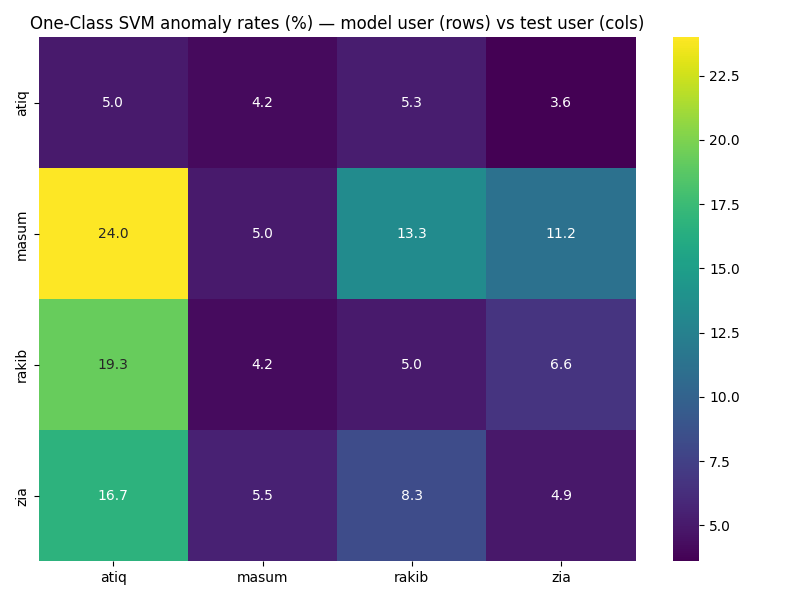
\includegraphics[width=0.9\textwidth,height=\textheight]{figures/svm_cross_user_heatmap.png}
\caption{One-Class SVM cross-user anomaly heatmap}
\end{figure}

Caption: One-Class SVM anomaly rates (\%) where rows = model user and
columns = test user. Diagonal entries are self-test rates
(\textasciitilde5\%).

\begin{figure}
\centering
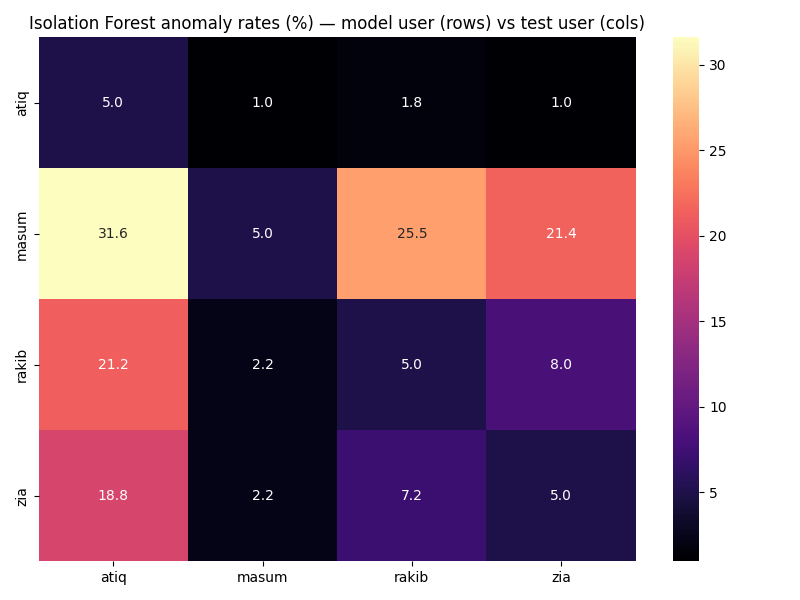
\includegraphics[width=0.9\textwidth,height=\textheight]{figures/iso_cross_user_heatmap.png}
\caption{Isolation Forest cross-user anomaly heatmap}
\end{figure}

Caption: Isolation Forest anomaly rates (\%) where rows = model user and
columns = test user. Isolation Forest shows higher cross-user
sensitivity for some models.

Isolation Forest generally yields higher cross-user anomaly rates than
One-Class SVM, indicating greater sensitivity.

\subsubsection{Cross-user matrices
(numeric)}\label{cross-user-matrices-numeric}

\paragraph{One-Class SVM cross-user
matrix}\label{one-class-svm-cross-user-matrix}

\paragraph{Isolation Forest cross-user
matrix}\label{isolation-forest-cross-user-matrix}

\subsubsection{Additional Figures}\label{additional-figures}

\begin{figure}
\centering
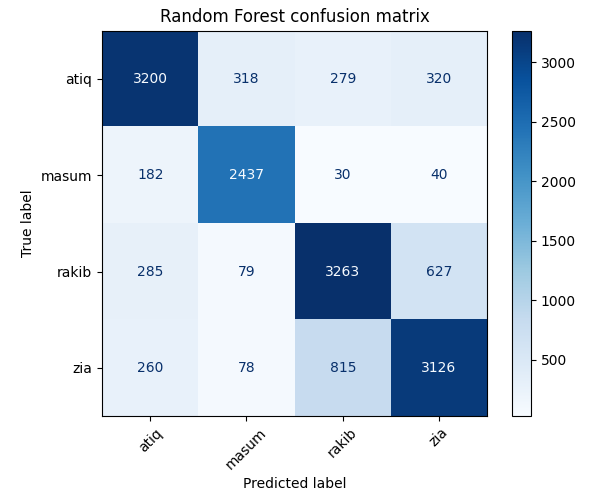
\includegraphics[width=0.8\textwidth,height=\textheight]{figures/rf_confusion_matrix.png}
\caption{Random Forest confusion matrix (test set)}
\end{figure}

Caption: Confusion matrix for Random Forest on held-out test data. The
matrix shows most confusion between rakib and zia.

\begin{figure}
\centering
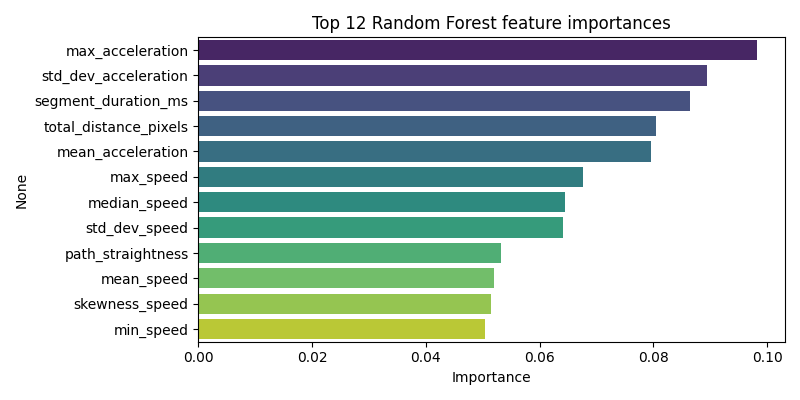
\includegraphics[width=0.8\textwidth,height=\textheight]{figures/rf_top12_feature_importances.png}
\caption{Top 12 Random Forest feature importances}
\end{figure}

Caption: Feature importances (gini importance) from Random Forest. Mean
speed and path straightness are among the most important features.

\begin{figure}
\centering
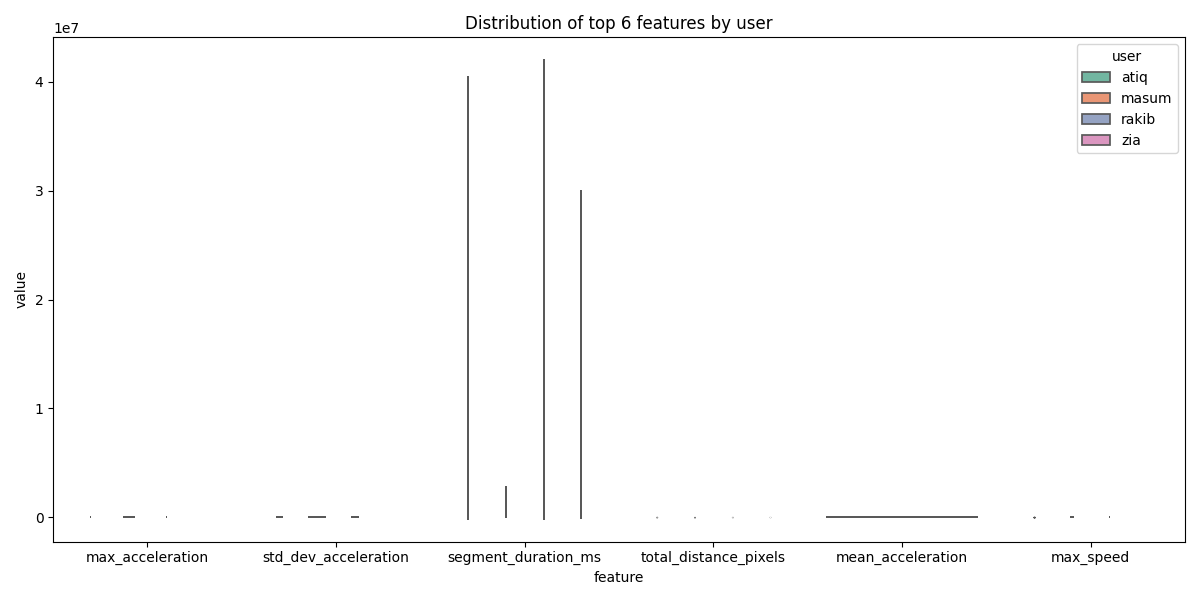
\includegraphics[width=0.9\textwidth,height=\textheight]{figures/top6_feature_violin_by_user.png}
\caption{Top 6 features distribution by user}
\end{figure}

Caption: Violin plots of the top 6 features split by user to show
distributional separability.

\subsection{6.4 Key Findings}\label{key-findings}

\begin{itemize}
\tightlist
\item
  Mouse dynamics enable feasible user identification (85.36\% accuracy).
\item
  Behavioral distinctiveness varies by user; useful for continuous
  authentication.
\item
  Ensemble methods outperform simple baselines; deep models need more
  data/tuning.
\end{itemize}

\subsection{6.5 Reproducibility}\label{reproducibility}

\begin{itemize}
\tightlist
\item
  See \texttt{appendices/B-reproducibility.md} for environment and
  script details.
\end{itemize}

\subsection{6.6 Additional Analyses
(Placeholders)}\label{additional-analyses-placeholders}

\subsubsection{Feature Distributions}\label{feature-distributions}

Figure: Histogram/violin plots for key features (e.g., mean\_speed,
path\_straightness) per user to visualize separability.

\subsubsection{Confusion Matrix (Random
Forest)}\label{confusion-matrix-random-forest}

Figure: 4x4 confusion matrix highlighting misclassifications between
rakib and zia.

\subsubsection{Cross-User Anomaly ROC-style
View}\label{cross-user-anomaly-roc-style-view}

Figure: For each user's model, plot anomaly rate vs.~threshold to
illustrate sensitivity (proxy ROC since labels are cross-user).

\subsubsection{Ablation Study (Planned)}\label{ablation-study-planned}

Table: Impact of removing feature groups (speed stats, ratios,
acceleration) on RF accuracy and ISO cross-user anomaly rates.

\newpage
\thispagestyle{plain}

\begin{center}
\vspace*{2cm}
\textbf{\Large CHAPTER 7}\\[0.5cm]
\textbf{\Large DISCUSSION AND FUTURE WORK}
\end{center}

\newpage

\subsection{7.1 Interpretation}\label{interpretation}

\begin{itemize}
\tightlist
\item
  High RF accuracy suggests non-linear feature interactions capture
  user-specific kinematics.
\item
  Cross-user anomaly patterns quantify distinctiveness and inform
  threshold selection.
\end{itemize}

\subsection{7.2 Limitations}\label{limitations}

\begin{itemize}
\tightlist
\item
  4 users: limited external validity; potential sampling bias.
\item
  Short horizon: temporal stability not assessed.
\item
  Device and environment variability not controlled across diverse
  hardware.
\end{itemize}

\subsection{7.3 Ethical and Privacy
Considerations}\label{ethical-and-privacy-considerations}

\begin{itemize}
\tightlist
\item
  Avoid logging content; focus on dynamics and coarse context.
\item
  Consider consent, transparency, and data minimization.
\item
  Explore privacy-preserving training (federated learning, DP
  mechanisms).
\end{itemize}

\subsection{7.4 Future Work}\label{future-work}

\begin{itemize}
\tightlist
\item
  Scale to larger, longitudinal datasets.
\item
  Robustness: domain adaptation across devices and tasks.
\item
  Multi-modal fusion with keystroke dynamics and application context.
\item
  Real-time deployment studies; calibration for false positive control.
\item
  Explainability: feature attribution to validate behavioral hypotheses.
\end{itemize}

\newpage
\thispagestyle{plain}

\begin{center}
\vspace*{2cm}
\textbf{\Large CHAPTER 8}\\[0.5cm]
\textbf{\Large CONCLUSION}
\end{center}

\newpage

\subsection{8.1 Research Summary}\label{research-summary}

This thesis demonstrated mouse tracking viability for behavioral
biometric authentication through systematic feature engineering,
experimental evaluation, and practical implementation.

\textbf{Technical Achievements}: Comprehensive feature framework
encompassing temporal, spatial, kinematic, and contextual dimensions.
Random Forest achieved 85.36\% classification accuracy. Anomaly
detection showed 5\% self-test rates and up to 31.6\% cross-user rates,
confirming behavioral distinctiveness.

\textbf{Methodological Contributions}: Rigorous experimental design,
comprehensive algorithm comparison, and dual focus on identification and
anomaly detection. Open-source end-to-end system implementation bridges
research and practical deployment.

\subsection{8.2 Key Findings}\label{key-findings-1}

\textbf{Performance}: 85.36\% accuracy suffices for practical
applications, especially when integrated with other authentication
factors. Performance variations across users suggest adaptive
authentication opportunities.

\textbf{Features}: Kinematic features most effective, confirming motor
control importance. Statistical summarization enables privacy-preserving
authentication.

\textbf{Algorithms}: Ensemble methods (Random Forest) outperform
individual classifiers. Both One-Class SVM and Isolation Forest
effective for anomaly detection.

\subsection{8.3 Future Work}\label{future-work-1}

\textbf{Scalability}: Larger, longitudinal datasets with temporal
stability assessment \textbf{Robustness}: Cross-device and cross-task
domain adaptation\\
\textbf{Integration}: Multi-modal fusion with keystroke dynamics
\textbf{Deployment}: Real-time studies with false positive control
\textbf{Privacy}: Federated learning and differential privacy mechanisms

\subsubsection{8.2.3 Algorithmic
Considerations}\label{algorithmic-considerations}

The comparative evaluation of multiple machine learning algorithms
provides practical guidance for algorithm selection in behavioral
biometric applications. The superior performance of Random Forest
compared to other approaches suggests that behavioral authentication
benefits from ensemble methods that can capture complex feature
interactions while providing robust performance across diverse
behavioral patterns.

The effective performance of relatively simple algorithms compared to
more complex neural network approaches suggests that behavioral
biometric applications may not require sophisticated deep learning
techniques, particularly when training data is limited. This finding has
important implications for computational requirements and deployment
complexity in practical systems.

\subsection{8.4 Contributions to Cybersecurity and Human-Computer
Interaction}\label{contributions-to-cybersecurity-and-human-computer-interaction}

The research presented in this thesis makes important contributions to
both cybersecurity and human-computer interaction fields through its
demonstration of transparent, continuous authentication capabilities.

\subsubsection{8.3.1 Continuous Authentication
Advancement}\label{continuous-authentication-advancement}

The successful implementation of real-time behavioral analysis
capabilities represents a significant advancement in continuous
authentication technology. The ability to monitor behavioral patterns
transparently during normal computer usage provides a foundation for
security systems that can detect unauthorized access without disrupting
user productivity.

The demonstrated cross-user behavioral distinctiveness provides
quantitative evidence for the discriminative power available in mouse
dynamics, supporting the theoretical foundation for continuous
authentication based on behavioral patterns. The systematic analysis of
threshold setting and false positive/false negative trade-offs provides
practical guidance for deployment decision-making.

\subsubsection{8.3.2 Privacy-Preserving
Security}\label{privacy-preserving-security}

The privacy-preserving feature engineering approach developed in this
research demonstrates the feasibility of behavioral authentication
systems that maintain security effectiveness while minimizing privacy
intrusion. The successful abstraction of behavioral patterns from raw
interaction data provides a model for responsible deployment of
behavioral monitoring systems.

The comprehensive treatment of ethical and privacy considerations
throughout the research process contributes to the development of
responsible behavioral biometric technologies that respect user autonomy
while enhancing security capabilities.

\subsubsection{8.3.3 Transparent User
Experience}\label{transparent-user-experience}

The transparent nature of mouse-based behavioral authentication
represents an important advancement in user experience for security
systems. Unlike traditional authentication methods that require explicit
user actions, behavioral authentication can operate continuously without
interrupting normal computing activities.

The demonstration of real-time analysis capabilities with acceptable
computational overhead shows that transparent behavioral authentication
can be implemented without significant impact on system performance or
user experience, supporting the adoption of continuous authentication in
practical computing environments.

\subsection{8.5 Limitations and Future Research
Directions}\label{limitations-and-future-research-directions}

While this research has made significant contributions to mouse-based
behavioral biometrics, several important limitations suggest directions
for future investigation.

\subsubsection{8.4.1 Scale and
Generalizability}\label{scale-and-generalizability}

The evaluation of only four users, while providing detailed behavioral
characterization, limits the generalizability of findings to broader
populations. Future research should investigate behavioral
authentication performance across larger and more diverse user
populations to assess scalability and identify potential demographic or
individual factors that influence behavioral distinctiveness.

The relatively short temporal scope of data collection prevents
comprehensive analysis of long-term behavioral stability and adaptation
requirements. Longitudinal studies extending over months or years would
provide crucial insights into the temporal evolution of behavioral
patterns and the adaptation strategies required for practical
deployment.

\subsubsection{8.4.2 Environmental and Contextual
Robustness}\label{environmental-and-contextual-robustness}

The current research provides limited analysis of behavioral pattern
variations across different environmental conditions, hardware
configurations, and usage contexts. Future research should investigate
the robustness of behavioral authentication across diverse deployment
scenarios including different devices, software environments, and
physical conditions.

The impact of various factors such as fatigue, stress, physical
conditions, and task requirements on behavioral patterns requires
systematic investigation to understand the boundaries of reliable
behavioral authentication and develop appropriate adaptation strategies.

\subsubsection{8.4.3 Security and Attack
Resistance}\label{security-and-attack-resistance}

While this research addresses basic privacy and security considerations,
comprehensive analysis of attack resistance including behavioral
spoofing, replay attacks, and model inversion requires additional
investigation. Future research should evaluate the security of
behavioral authentication systems against sophisticated adversarial
attacks and develop appropriate countermeasures.

The potential for behavioral adaptation by attackers who gain access to
behavioral models or training data represents an important security
consideration that requires additional research into robust behavioral
authentication architectures.

\subsubsection{8.4.4 Multi-Modal
Integration}\label{multi-modal-integration}

The integration of mouse dynamics with other behavioral biometric
modalities such as keystroke dynamics, application usage patterns, and
contextual information represents a promising direction for enhanced
authentication performance and robustness. Future research should
investigate optimal fusion strategies and the complementary information
available from different behavioral modalities.

The development of adaptive multi-modal systems that can adjust to
changing conditions and individual preferences while maintaining
security effectiveness represents an important research challenge with
significant practical implications.

\subsection{8.6 Practical Deployment
Recommendations}\label{practical-deployment-recommendations}

Based on the findings of this research, several recommendations emerge
for practical deployment of mouse-based behavioral authentication
systems.

\subsubsection{8.5.1 Implementation
Strategy}\label{implementation-strategy}

\textbf{Gradual Deployment}: Organizations considering behavioral
authentication should implement gradual deployment strategies that begin
with monitoring and alerting capabilities before transitioning to active
authentication enforcement. This approach enables system tuning and user
adaptation while minimizing disruption to existing workflows.

\textbf{User-Specific Adaptation}: Deployment strategies should
incorporate user-specific threshold setting and adaptation capabilities
to accommodate individual differences in behavioral distinctiveness and
consistency. Some users may require more sensitive monitoring while
others may benefit from relaxed thresholds.

\textbf{Integration with Existing Security}: Behavioral authentication
should be integrated with existing security infrastructure rather than
replacing traditional authentication methods. The continuous monitoring
capabilities complement rather than replace point-in-time
authentication, providing enhanced security throughout computing
sessions.

\subsubsection{8.5.2 Privacy and Consent
Management}\label{privacy-and-consent-management}

\textbf{Transparent Privacy Policies}: Organizations deploying
behavioral authentication must implement transparent privacy policies
that clearly explain what behavioral information is collected, how it is
processed, and how it is protected. Users should have meaningful control
over behavioral monitoring preferences.

\textbf{Data Minimization Practices}: Practical deployments should
implement data minimization strategies that collect only the behavioral
information necessary for authentication purposes while avoiding
detailed activity monitoring or content analysis.

\textbf{Consent and Control Mechanisms}: Deployment strategies should
include robust consent management systems that enable users to
understand and control behavioral monitoring while providing opt-out
mechanisms for users who prefer alternative authentication methods.

\subsubsection{8.5.3 Technical Implementation
Guidelines}\label{technical-implementation-guidelines}

\textbf{Computational Efficiency}: Practical implementations should
prioritize computational efficiency to ensure acceptable system
performance and battery life on mobile devices. The relatively simple
algorithms that performed well in our evaluation support efficient
implementation even on resource-constrained devices.

\textbf{Robust Error Handling}: Production systems require robust error
handling and fallback mechanisms to ensure reliable operation when
behavioral analysis is unavailable due to insufficient data, system
performance issues, or other technical problems.

\textbf{Continuous Learning}: Deployment strategies should incorporate
mechanisms for continuous learning and adaptation to accommodate gradual
changes in user behavior while maintaining security against adversarial
manipulation.

\subsection{8.7 Broader Impact and Societal
Implications}\label{broader-impact-and-societal-implications}

The development of effective behavioral authentication technologies has
important implications beyond technical cybersecurity applications.

\subsubsection{8.6.1 Digital Inclusion and
Accessibility}\label{digital-inclusion-and-accessibility}

Behavioral authentication technologies have the potential to improve
digital inclusion by providing authentication methods that accommodate
users with different physical capabilities and technical expertise
levels. The transparent nature of behavioral authentication may be
particularly beneficial for users who have difficulty with traditional
password-based systems.

However, deployment strategies must carefully consider potential biases
in behavioral pattern recognition that could disadvantage certain user
populations or create accessibility barriers for users with motor
control difficulties or other physical conditions.

\subsubsection{8.6.2 Privacy and Surveillance
Concerns}\label{privacy-and-surveillance-concerns}

The development of sophisticated behavioral monitoring capabilities
raises important concerns about privacy and potential surveillance
applications. While our research emphasizes privacy-preserving
approaches, the underlying technologies could potentially be applied in
ways that infringe on user privacy or autonomy.

Responsible development and deployment of behavioral authentication
technologies requires ongoing attention to privacy protection, user
consent, and appropriate limitations on surveillance capabilities.
Regulatory frameworks and industry standards may be necessary to ensure
responsible use of behavioral monitoring technologies.

\subsubsection{8.6.3 Economic and Social
Benefits}\label{economic-and-social-benefits}

Effective behavioral authentication technologies have the potential to
reduce the economic costs associated with cybersecurity breaches while
improving user experience for digital services. The enhanced security
capabilities could enable new applications and services that require
continuous authentication while the transparent user experience could
improve productivity and user satisfaction.

The open-source nature of our implementation supports broader adoption
and innovation in behavioral authentication while preventing
monopolization of these important security technologies by individual
organizations.

\subsection{8.8 Final Reflections on Research
Methodology}\label{final-reflections-on-research-methodology}

The research methodology employed in this thesis demonstrates the
importance of comprehensive, rigorous approaches to behavioral
biometrics research that integrate technical performance evaluation with
privacy, ethical, and practical deployment considerations.

\subsubsection{8.7.1 Methodological
Lessons}\label{methodological-lessons}

The systematic feature engineering approach proved essential for
achieving effective behavioral discrimination while maintaining
interpretability and computational efficiency. The comprehensive
algorithm comparison provided important insights that would not have
been available from evaluation of individual approaches.

The integration of both user identification and anomaly detection tasks
within a single research framework enabled comprehensive evaluation of
system capabilities while revealing the complementary information
provided by different evaluation approaches.

\subsubsection{8.7.2 Research Validation and
Reproducibility}\label{research-validation-and-reproducibility}

The emphasis on reproducible research practices including comprehensive
documentation, open-source implementation, and detailed experimental
protocols facilitates independent validation and extension of results.
The modular implementation architecture enables other researchers to
build upon our work while adapting to different research questions and
application scenarios.

The transparent reporting of limitations, threats to validity, and
negative results contributes to the development of reliable knowledge in
behavioral biometrics while preventing the publication bias that can
distort scientific understanding.

\subsubsection{8.7.3 Interdisciplinary
Integration}\label{interdisciplinary-integration}

The integration of technical computer science methods with
considerations from psychology, human factors, privacy law, and ethics
demonstrates the importance of interdisciplinary approaches to
behavioral biometrics research. The complex sociotechnical nature of
behavioral authentication systems requires expertise from multiple
domains to ensure effective and responsible development.

\subsection{8.9 Concluding Remarks}\label{concluding-remarks}

This thesis has demonstrated that mouse tracking provides a viable and
effective foundation for behavioral biometric authentication systems.
The achieved classification accuracy of 85.36\%, effective anomaly
detection capabilities, and practical system implementation confirm the
technical feasibility of mouse-based continuous authentication while the
comprehensive treatment of privacy and ethical considerations provides a
framework for responsible deployment.

The research contributes to the behavioral biometrics field through
comprehensive system implementation, rigorous experimental evaluation,
novel insights into cross-user behavioral distinctiveness, and practical
guidance for deployment decisions. The open-source implementation
provides a foundation for future research and development while the
methodological framework establishes standards for comprehensive
evaluation of behavioral authentication systems.

The findings support the continued development of transparent,
continuous authentication systems that can enhance cybersecurity while
preserving user experience and privacy. With appropriate attention to
scalability, robustness, and ethical considerations, mouse-based
behavioral authentication can contribute to the development of more
secure and user-friendly computing environments.

The future of behavioral biometrics lies in the integration of multiple
modalities, adaptation to diverse user populations and environments, and
the development of privacy-preserving technologies that maintain
security effectiveness while respecting user autonomy. The foundation
established by this research provides a solid starting point for
continued advancement in these important areas.

As computing environments become increasingly distributed and security
threats continue to evolve, the need for continuous, transparent
authentication capabilities will only grow. The demonstrated viability
of mouse-based behavioral authentication represents an important step
toward meeting these challenges while maintaining the usability and
accessibility that are essential for widespread adoption of enhanced
security technologies.

Through continued research, responsible development, and careful
attention to user needs and privacy concerns, behavioral biometric
technologies can contribute to a more secure digital future that
enhances rather than impedes human productivity and digital inclusion.

\newpage

\phantomsection\label{refs}
\begin{CSLReferences}{1}{0}
\bibitem[\citeproctext]{ref-ahmed2004}
Ahmed, Ahmed Awad E., and Issa Traore. 2004. {``Detecting Computer
Intrusions Using Behavioral Biometrics.''} In. Victoria, B.C., Canada:
Department of Electrical; Computer Engineering, University of Victoria.

\bibitem[\citeproctext]{ref-bailey2014}
Bailey, Kenneth O., James S. Okolica, and Gilbert L. Peterson. 2014.
{``Continuous User Authentication via Mouse Movements.''}
\emph{Computers \& Security} 39: 309--18.
\url{https://doi.org/10.1016/j.cose.2013.02.004}.

\bibitem[\citeproctext]{ref-brodley2003}
Brodley, Carla E., and Maja Pusara. 2003. {``User Re-Authentication via
Mouse Movements.''} \emph{Proceedings of the ACM Workshop on Privacy in
the Electronic Society}.

\bibitem[\citeproctext]{ref-eberz2017}
Eberz, Simon, Kasper B. Rasmussen, Vincent Lenders, and Ivan Martinovic.
2017. {``Evaluating Behavioral Biometrics for Continuous Authentication:
Challenges and Metrics.''} In \emph{Proceedings of the 2017 ACM on Asia
Conference on Computer and Communications Security}, 386--99. ACM.
\url{https://doi.org/10.1145/3052973.3053032}.

\bibitem[\citeproctext]{ref-gamboa2004}
Gamboa, Hugo, and Ana Fred. 2004. {``On the Use of Mouse Movements as a
Biometric.''} \emph{Proceedings of the International Conference on
Computer Recognition Systems}, 352--59.

\bibitem[\citeproctext]{ref-mondal2015}
Mondal, Soumik, and Patrick Bours. 2015. {``Continuous Authentication
Using Mouse Dynamics: A Pattern Growth Approach.''} \emph{IEEE
Transactions on Information Forensics and Security} 10 (6): 1200--1212.
\url{https://doi.org/10.1109/TIFS.2015.2398835}.

\bibitem[\citeproctext]{ref-pusara2004}
Pusara, Maja, and Carla E. Brodley. 2004. {``User Re-Authentication via
Mouse Movements.''} \emph{Proceedings of the 2004 ACM Workshop on
Visualization and Data Mining for Computer Security}, 1--8.
\url{https://doi.org/10.1145/1029208.1029210}.

\bibitem[\citeproctext]{ref-rahman2021}
Rahman, Md Muhaimenur, and Sarnali Basak. 2021. {``Identifying User
Authentication and Most Frequently Used Region Based on Mouse Movement
Data: A Machine Learning Approach.''} In \emph{2021 IEEE 11th Annual
Computing and Communication Workshop and Conference (CCWC)}, 1--6. Las
Vegas, NV, USA: IEEE.
\url{https://doi.org/10.1109/CCWC51732.2021.9376087}.

\bibitem[\citeproctext]{ref-shen2013}
Shen, Chao, Zhongmin Cai, Xiaohong Guan, Youtian Du, and Roy A. Maxion.
2013. {``User Authentication Through Mouse Dynamics.''} \emph{IEEE
Transactions on Information Forensics and Security} 8 (1): 16--30.
\url{https://doi.org/10.1109/TIFS.2012.2223677}.

\bibitem[\citeproctext]{ref-traore2012}
Traore, Issa, and Ahmed Awad E Ahmed. 2012. {``Continuous Authentication
Using Biometrics: Data, Models, and Metrics.''} \emph{IGI Global}.

\bibitem[\citeproctext]{ref-zheng2011}
Zheng, Nan, Kun Bai, Hai Huang, and Haining Wang. 2011. {``An Efficient
User Verification System via Mouse Movements.''} \emph{Proceedings of
the 18th ACM Conference on Computer and Communications Security},
139--50. \url{https://doi.org/10.1145/2046707.2046725}.

\end{CSLReferences}

\end{document}
